% Gemini 3.1 Pro's 10/10 Multi-Head Attention Figure
% This is the target output quality for Relic
\documentclass[border=5mm]{standalone}
\usepackage{tikz}
\usepackage{amsmath}
\usetikzlibrary{positioning, fit, backgrounds, arrows.meta, shadows.blur, calc, shapes.geometric}

\begin{document}
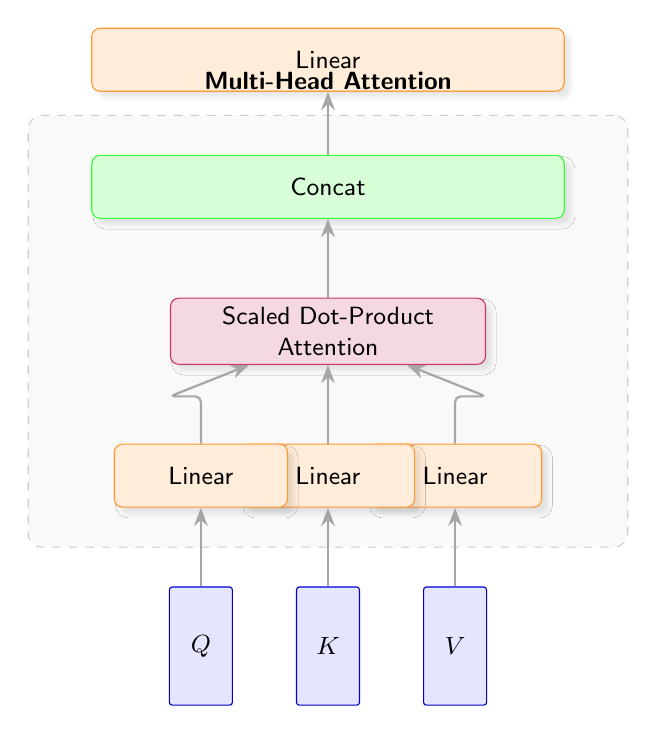
\begin{tikzpicture}[
  font=\sffamily\small,
  >=Stealth,
  relicbox/.style={rectangle, draw=gray!80, fill=white, rounded corners=3pt, minimum width=22mm, minimum height=8mm, align=center, blur shadow={shadow blur steps=5, shadow opacity=10}},
  relictensor/.style={rectangle, draw=blue!80!black, fill=blue!10, rounded corners=1pt, minimum width=8mm, minimum height=15mm},
  relicop/.style={circle, draw=gray!80, fill=white, inner sep=1pt, minimum size=6mm},
  relicarrow/.style={->, thick, draw=gray!70, rounded corners=2pt},
  busline/.style={-, thick, draw=gray!70, rounded corners=2pt}
]

% Data Inputs (Tensors)
\node[relictensor] (V) {$V$};
\node[relictensor, left=8mm of V] (K) {$K$};
\node[relictensor, left=8mm of K] (Q) {$Q$};

% Linear Layers
\node[relicbox, fill=orange!15, draw=orange!80, above=10mm of V] (LinV) {Linear};
\node[relicbox, fill=orange!15, draw=orange!80, above=10mm of K] (LinK) {Linear};
\node[relicbox, fill=orange!15, draw=orange!80, above=10mm of Q] (LinQ) {Linear};

% Scaled Dot Product
\node[relicbox, fill=purple!15, draw=purple!80, above=10mm of LinK, minimum width=40mm] (SDP) {Scaled Dot-Product\\Attention};

% Concat & Final Linear
\node[relicbox, fill=green!15, draw=green!80, above=10mm of SDP, minimum width=60mm] (Concat) {Concat};
\node[relicbox, fill=orange!15, draw=orange!80, above=8mm of Concat, minimum width=60mm] (LinFinal) {Linear};

% Grouping
\begin{scope}[on background layer]
  \node[draw=gray!40, dashed, fill=gray!5, rounded corners=5pt, inner xsep=8mm, inner ysep=5mm, fit=(LinV) (LinQ) (Concat)] (MHA_Container) {};
\end{scope}
\node[above=2mm of MHA_Container.north] {\textbf{Multi-Head Attention}};

% Routing
\draw[relicarrow] (V) -- (LinV);
\draw[relicarrow] (K) -- (LinK);
\draw[relicarrow] (Q) -- (LinQ);

% Routing into SDP
\draw[relicarrow] (LinV.north) |- ([yshift=-4mm]SDP.south east) -- ([xshift=10mm]SDP.south);
\draw[relicarrow] (LinK.north) -- (SDP.south);
\draw[relicarrow] (LinQ.north) |- ([yshift=-4mm]SDP.south west) -- ([xshift=-10mm]SDP.south);

% Routing out
\draw[relicarrow] (SDP.north) -- (Concat.south);
\draw[relicarrow] (Concat.north) -- (LinFinal.south);

\end{tikzpicture}
\end{document}
